%/*
% * SPDX-FileCopyrightText: 2021 Stefan Begerad <stefan@begerad.de>
% *
% * SPDX-License-Identifier: GPL-3.0-or-later
% */

%make document a Beamer presentaion
\documentclass{beamer}

%include preamble
%/*
% * SPDX-FileCopyrightText: 2021 Stefan Begerad <stefan@begerad.de>
% *
% * SPDX-License-Identifier: GPL-3.0-or-later
% */

%define outer theme (color and background)
%\usetheme{default}
%\usetheme{Goettingen}
%\usetheme{Darmstadt}
%\usetheme{Copenhagen}
\usetheme{Boadilla}
%\usetheme{Berlin}
%\usetheme{Berkeley}
%\usetheme{Bergen}
%\usetheme{Antibes}
%\usetheme{AnnArbor}
%\usetheme{Warsaw}
%\usetheme{Szeged}

%define color of theme
%\usecolortheme{default}
%\usecolortheme{beaver}
\usecolortheme{seahorse}

%add the following package to use links
%Define hyperref as last package, because it modifies other instructions!
\usepackage{hyperref}

\title[Dede]%optional
{Dede Echtzeit-Karte}

\subtitle{Offen, Unabhängig, Universell}

\author[Begerad]%(optional, for multiple authors)
{Stefan~Begerad}

\date[OTM, 6.2.2021]%(optional)
{Open Transport Meetup, June 2. 2021}

\logo{
\includegraphics[height=1cm]{dede/dedeLogo0128}}


%define the document
\begin{document}

%define title page
\begin{frame}
  \titlepage
\end{frame}

%outline table of content for the entire presentation
%use asterisk to indicate that this section shall not be part of the table
%the name of the section serves as the title of the slide
\AtBeginSection[]
{
    \begin{frame}
        \frametitle{Inhalt}
        \tableofcontents[currentsection]
    \end{frame}
}

\section{gtfsvtor}

%/*
% * SPDX-FileCopyrightText: 2021 Stefan Begerad <stefan@begerad.de>
% *
% * SPDX-License-Identifier: GPL-3.0-or-later
% */

\begin{frame}{Gtfsvtor Usage}
  \begin{itemize}
  \item Instruction call:
    \begin{itemize}
    \item ./Gtfsvtor/bin/Gtfsvtor --numThreads 2 -o validation-results-vbn-top-dhid-2021-09-07.html ~/gtfs/vbn/top-level-dhid/pxypihdrpv\_connect-only\_top\_level\_stops-DHID.zip
    \end{itemize}
  \end{itemize}
\end{frame}

\begin{frame}{Gtfsvtor Report Summary}
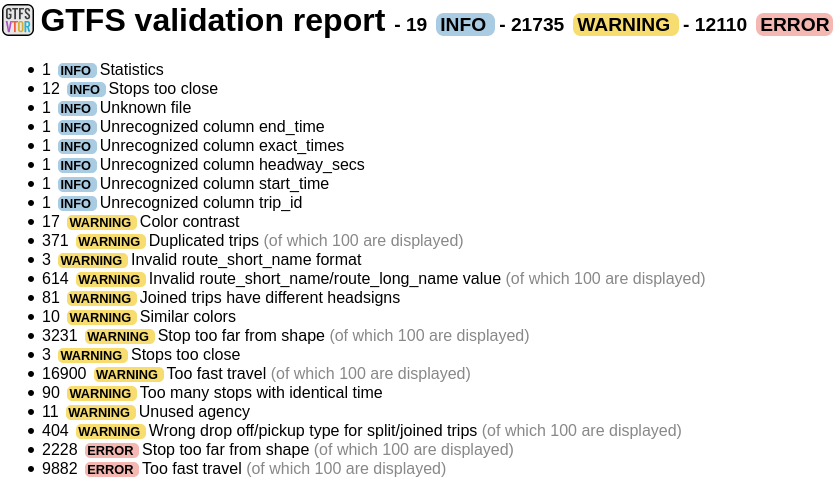
\includegraphics[width=0.95\paperwidth]{gtfs-validation/gtfsvtor-report-vbn-top-dhid.png}
\end{frame}

\begin{frame}{Gtfsvtor Unknown File}
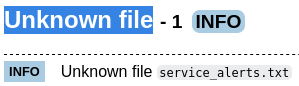
\includegraphics[width=0.5\textwidth]{gtfs-validation/gtfsvtor-report-vbn-top-dhid-unknown-file.png}
\end{frame}

\begin{frame}{GTFS File Requirements}
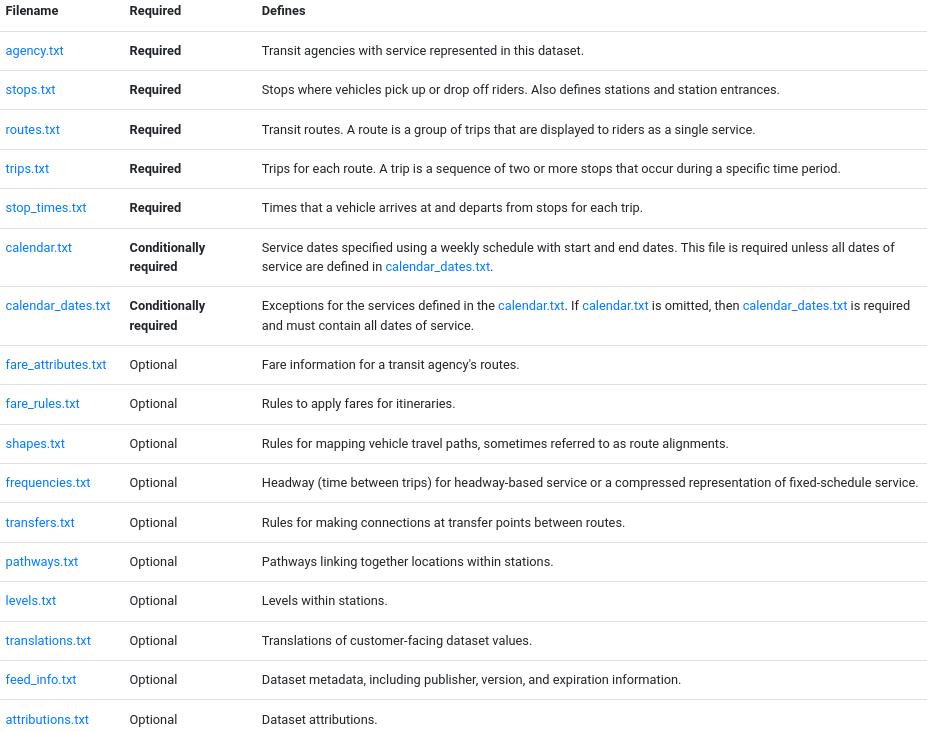
\includegraphics[width=0.95\paperwidth]{gtfs-validation/gtfs-spec-file-requirements.png}
\end{frame}

\begin{frame}{Gtfsvtor Too Fast Travel}
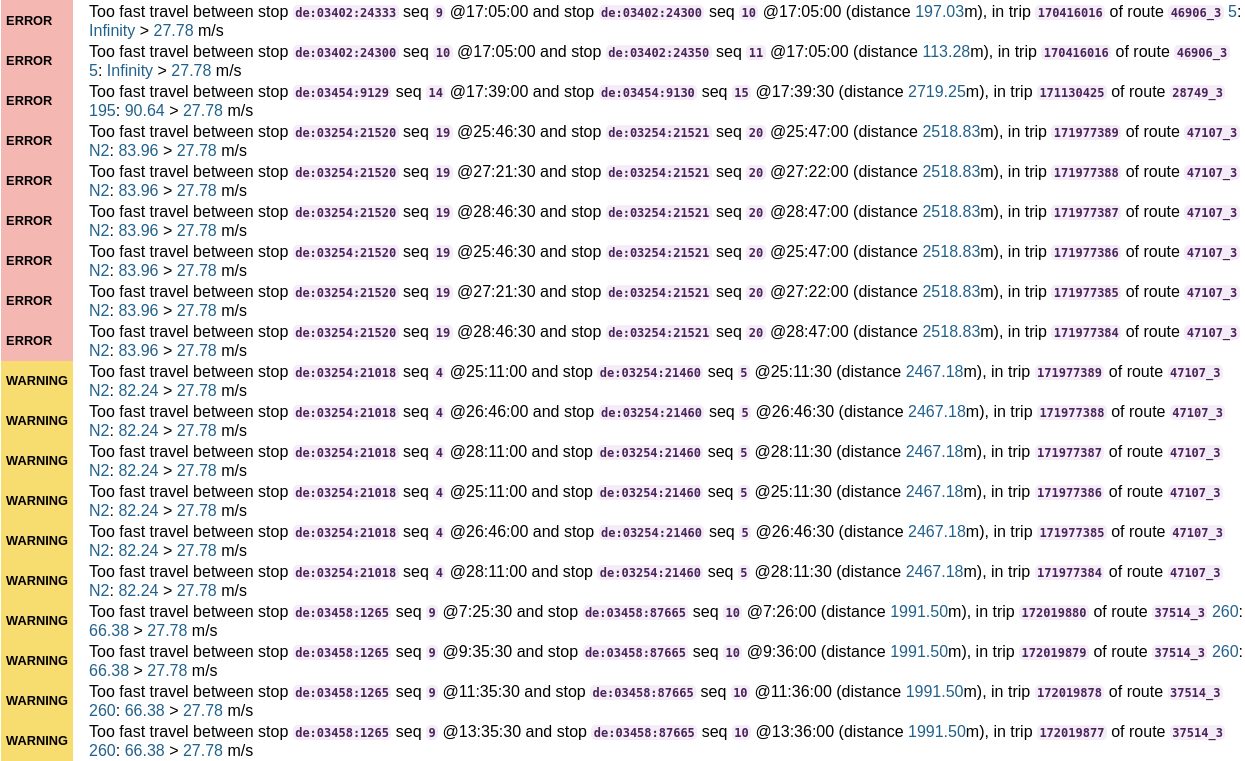
\includegraphics[width=0.95\paperwidth]{gtfs-validation/gtfsvtor-report-vbn-top-dhid-too-fast.png}
\end{frame}

\begin{frame}{Gtfsvtor Invalid route\_short\_name Value/Format}
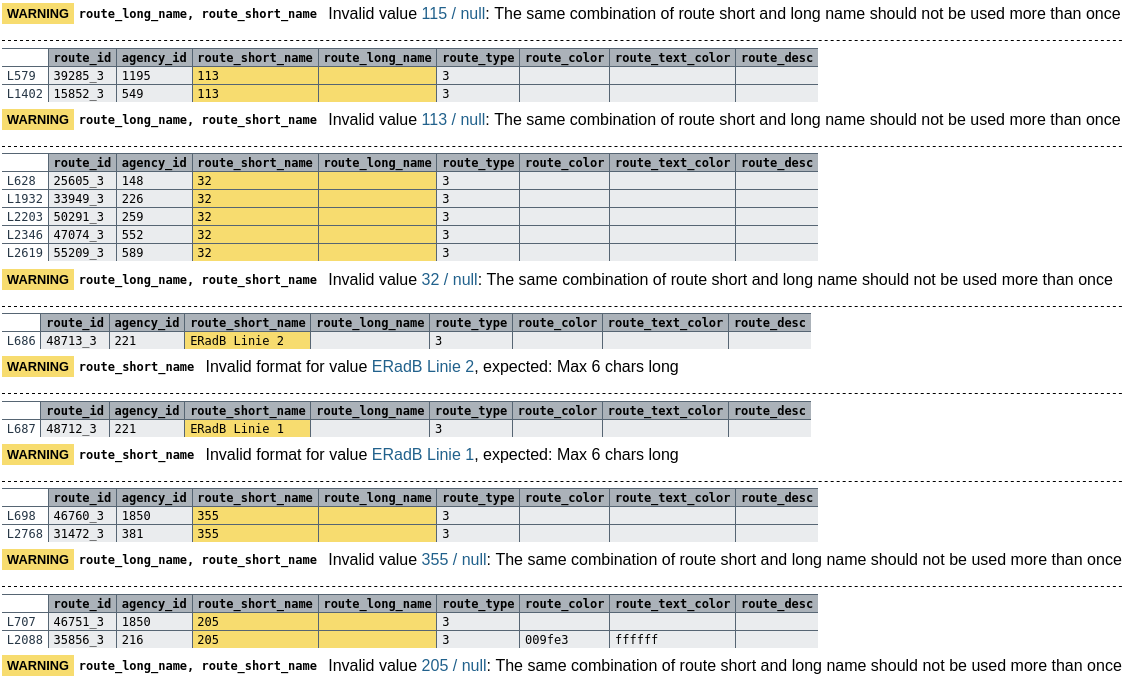
\includegraphics[width=0.95\paperwidth]{gtfs-validation/gtfsvtor-report-vbn-top-dhid-invalid.png}
\end{frame}

\begin{frame}{Gtfsvtor Stops too ...}
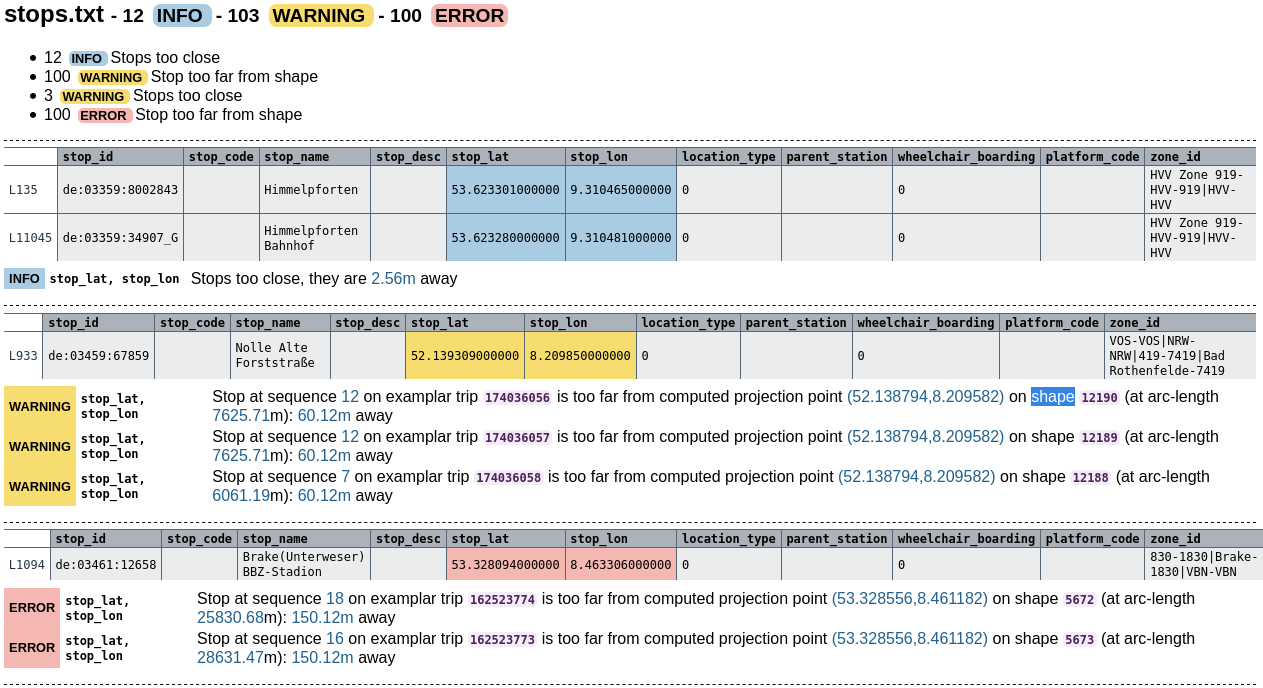
\includegraphics[width=0.95\paperwidth]{gtfs-validation/gtfsvtor-report-vbn-top-dhid-stops-too.png}
\end{frame}

\begin{frame}{Gtfsvtor Too Many Stops With Identical Time}
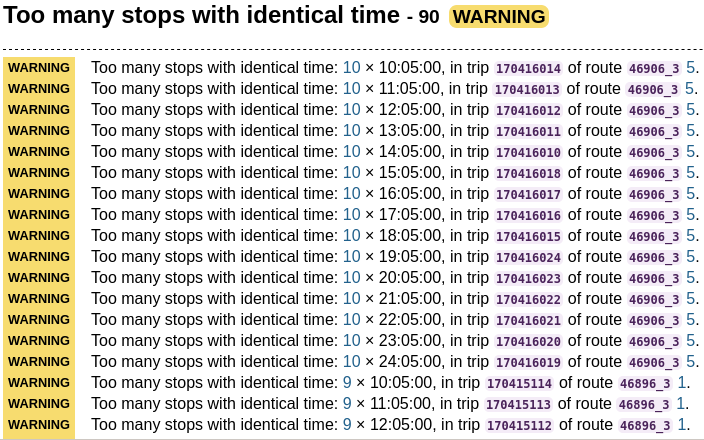
\includegraphics[width=0.9\paperwidth]{gtfs-validation/gtfsvtor-report-vbn-top-dhid-identical-time.png}
\end{frame}


\section{gtfs-validator}

%/*
% * SPDX-FileCopyrightText: 2021 Stefan Begerad <stefan@begerad.de>
% *
% * SPDX-License-Identifier: GPL-3.0-or-later
% */

\begin{frame}{Gtfs-validator Usage}
  \begin{itemize}
  \item Instruction call:
    \begin{itemize}
      \item java -jar gtfs-validator-v2.0.0\_cli.jar -u http://www.connect-info.net/opendata/gtfs/connect-nds-toplevel-dhid/pxypihdrpv --output\_base vbn-top-dhid-vl-rp-3 --feed\_name de-vbn -t 2
    \end{itemize}
  \end{itemize}
\end{frame}

\begin{frame}{Gtfs-validator Report Summary}
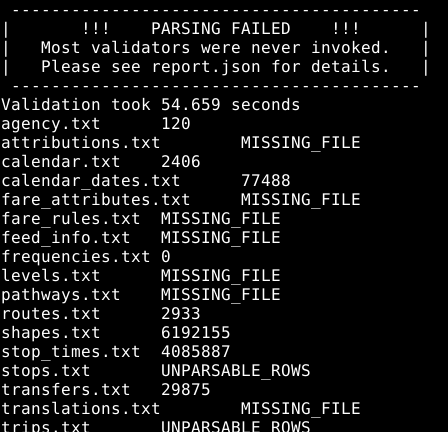
\includegraphics[width=0.6\textwidth]{gtfs-validation/gtfs-validator-report-summary.png}
\end{frame}

\begin{frame}{Gtfs-validator Whitespaces}
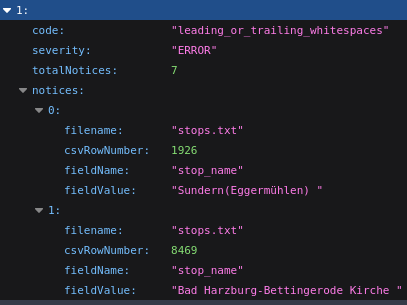
\includegraphics[width=0.75\textwidth]{gtfs-validation/gtfs-validator-report-whitespaces.png}
\end{frame}

\begin{frame}{Gtfs-validator route\_short\_name Too Long}
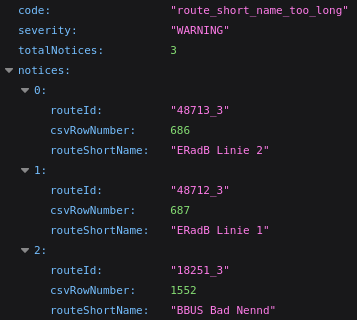
\includegraphics[width=0.75\textwidth]{gtfs-validation/gtfs-validator-report-short-name-too-long.png}
\end{frame}


\begin{frame}{Cheers!}
  \center {\Huge\textbf{Questions?}}
\end{frame}

\end{document}
k
